% Created by tikzDevice version 0.10.1 on 2017-12-04 15:15:24
% !TEX encoding = UTF-8 Unicode
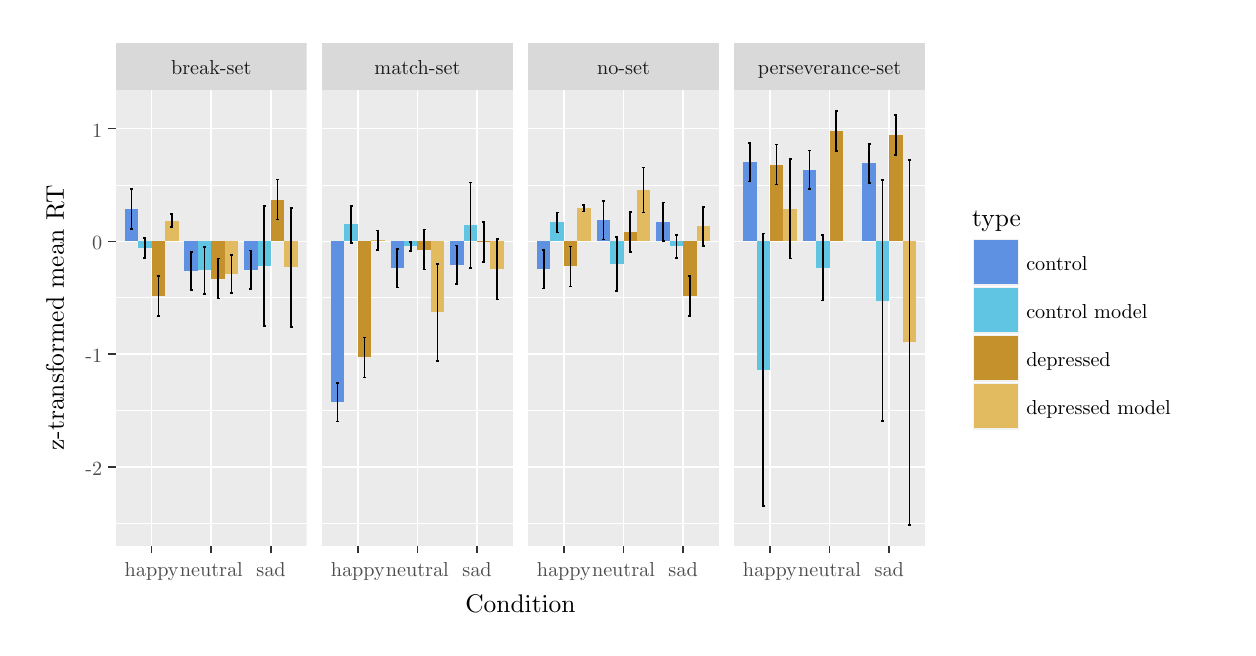
\begin{tikzpicture}[x=1pt,y=1pt]
\definecolor{fillColor}{RGB}{255,255,255}
\path[use as bounding box,fill=fillColor,fill opacity=0.00] (0,0) rectangle (433.62,216.81);
\begin{scope}
\path[clip] (  0.00,  0.00) rectangle (433.62,216.81);
\definecolor{drawColor}{RGB}{255,255,255}
\definecolor{fillColor}{RGB}{255,255,255}

\path[draw=drawColor,line width= 0.6pt,line join=round,line cap=round,fill=fillColor] (  0.00,  0.00) rectangle (433.62,216.81);
\end{scope}
\begin{scope}
\path[clip] ( 31.87, 29.59) rectangle (100.84,194.25);
\definecolor{fillColor}{gray}{0.92}

\path[fill=fillColor] ( 31.87, 29.59) rectangle (100.84,194.25);
\definecolor{drawColor}{RGB}{255,255,255}

\path[draw=drawColor,line width= 0.3pt,line join=round] ( 31.87, 37.80) --
	(100.84, 37.80);

\path[draw=drawColor,line width= 0.3pt,line join=round] ( 31.87, 78.52) --
	(100.84, 78.52);

\path[draw=drawColor,line width= 0.3pt,line join=round] ( 31.87,119.24) --
	(100.84,119.24);

\path[draw=drawColor,line width= 0.3pt,line join=round] ( 31.87,159.96) --
	(100.84,159.96);

\path[draw=drawColor,line width= 0.6pt,line join=round] ( 31.87, 58.16) --
	(100.84, 58.16);

\path[draw=drawColor,line width= 0.6pt,line join=round] ( 31.87, 98.88) --
	(100.84, 98.88);

\path[draw=drawColor,line width= 0.6pt,line join=round] ( 31.87,139.60) --
	(100.84,139.60);

\path[draw=drawColor,line width= 0.6pt,line join=round] ( 31.87,180.32) --
	(100.84,180.32);

\path[draw=drawColor,line width= 0.6pt,line join=round] ( 44.80, 29.59) --
	( 44.80,194.25);

\path[draw=drawColor,line width= 0.6pt,line join=round] ( 66.36, 29.59) --
	( 66.36,194.25);

\path[draw=drawColor,line width= 0.6pt,line join=round] ( 87.91, 29.59) --
	( 87.91,194.25);
\definecolor{fillColor}{RGB}{226,186,95}

\path[fill=fillColor] ( 49.65,139.60) rectangle ( 54.50,147.10);
\definecolor{fillColor}{RGB}{196,145,45}

\path[fill=fillColor] ( 44.80,119.96) rectangle ( 49.65,139.60);
\definecolor{fillColor}{RGB}{95,197,226}

\path[fill=fillColor] ( 39.95,137.17) rectangle ( 44.80,139.60);
\definecolor{fillColor}{RGB}{95,145,226}

\path[fill=fillColor] ( 35.10,139.60) rectangle ( 39.95,151.28);
\definecolor{fillColor}{RGB}{226,186,95}

\path[fill=fillColor] ( 71.21,127.71) rectangle ( 76.06,139.60);
\definecolor{fillColor}{RGB}{196,145,45}

\path[fill=fillColor] ( 66.36,126.15) rectangle ( 71.21,139.60);
\definecolor{fillColor}{RGB}{95,197,226}

\path[fill=fillColor] ( 61.51,129.13) rectangle ( 66.36,139.60);
\definecolor{fillColor}{RGB}{95,145,226}

\path[fill=fillColor] ( 56.66,128.88) rectangle ( 61.51,139.60);
\definecolor{fillColor}{RGB}{226,186,95}

\path[fill=fillColor] ( 92.76,130.15) rectangle ( 97.61,139.60);
\definecolor{fillColor}{RGB}{196,145,45}

\path[fill=fillColor] ( 87.91,139.60) rectangle ( 92.76,154.70);
\definecolor{fillColor}{RGB}{95,197,226}

\path[fill=fillColor] ( 83.06,130.72) rectangle ( 87.91,139.60);
\definecolor{fillColor}{RGB}{95,145,226}

\path[fill=fillColor] ( 78.21,129.34) rectangle ( 83.06,139.60);
\definecolor{drawColor}{RGB}{0,0,0}

\path[draw=drawColor,line width= 0.6pt,line join=round] ( 51.54,149.42) --
	( 52.62,149.42);

\path[draw=drawColor,line width= 0.6pt,line join=round] ( 52.08,149.42) --
	( 52.08,144.78);

\path[draw=drawColor,line width= 0.6pt,line join=round] ( 51.54,144.78) --
	( 52.62,144.78);

\path[draw=drawColor,line width= 0.6pt,line join=round] ( 46.69,127.19) --
	( 47.77,127.19);

\path[draw=drawColor,line width= 0.6pt,line join=round] ( 47.23,127.19) --
	( 47.23,112.73);

\path[draw=drawColor,line width= 0.6pt,line join=round] ( 46.69,112.73) --
	( 47.77,112.73);

\path[draw=drawColor,line width= 0.6pt,line join=round] ( 41.84,140.82) --
	( 42.92,140.82);

\path[draw=drawColor,line width= 0.6pt,line join=round] ( 42.38,140.82) --
	( 42.38,133.52);

\path[draw=drawColor,line width= 0.6pt,line join=round] ( 41.84,133.52) --
	( 42.92,133.52);

\path[draw=drawColor,line width= 0.6pt,line join=round] ( 36.99,158.42) --
	( 38.07,158.42);

\path[draw=drawColor,line width= 0.6pt,line join=round] ( 37.53,158.42) --
	( 37.53,144.15);

\path[draw=drawColor,line width= 0.6pt,line join=round] ( 36.99,144.15) --
	( 38.07,144.15);

\path[draw=drawColor,line width= 0.6pt,line join=round] ( 73.09,134.59) --
	( 74.17,134.59);

\path[draw=drawColor,line width= 0.6pt,line join=round] ( 73.63,134.59) --
	( 73.63,120.82);

\path[draw=drawColor,line width= 0.6pt,line join=round] ( 73.09,120.82) --
	( 74.17,120.82);

\path[draw=drawColor,line width= 0.6pt,line join=round] ( 68.24,133.36) --
	( 69.32,133.36);

\path[draw=drawColor,line width= 0.6pt,line join=round] ( 68.78,133.36) --
	( 68.78,118.95);

\path[draw=drawColor,line width= 0.6pt,line join=round] ( 68.24,118.95) --
	( 69.32,118.95);

\path[draw=drawColor,line width= 0.6pt,line join=round] ( 63.39,137.65) --
	( 64.47,137.65);

\path[draw=drawColor,line width= 0.6pt,line join=round] ( 63.93,137.65) --
	( 63.93,120.60);

\path[draw=drawColor,line width= 0.6pt,line join=round] ( 63.39,120.60) --
	( 64.47,120.60);

\path[draw=drawColor,line width= 0.6pt,line join=round] ( 58.54,135.83) --
	( 59.62,135.83);

\path[draw=drawColor,line width= 0.6pt,line join=round] ( 59.08,135.83) --
	( 59.08,121.93);

\path[draw=drawColor,line width= 0.6pt,line join=round] ( 58.54,121.93) --
	( 59.62,121.93);

\path[draw=drawColor,line width= 0.6pt,line join=round] ( 94.65,151.75) --
	( 95.72,151.75);

\path[draw=drawColor,line width= 0.6pt,line join=round] ( 95.18,151.75) --
	( 95.18,108.55);

\path[draw=drawColor,line width= 0.6pt,line join=round] ( 94.65,108.55) --
	( 95.72,108.55);

\path[draw=drawColor,line width= 0.6pt,line join=round] ( 89.80,161.93) --
	( 90.87,161.93);

\path[draw=drawColor,line width= 0.6pt,line join=round] ( 90.33,161.93) --
	( 90.33,147.48);

\path[draw=drawColor,line width= 0.6pt,line join=round] ( 89.80,147.48) --
	( 90.87,147.48);

\path[draw=drawColor,line width= 0.6pt,line join=round] ( 84.95,152.42) --
	( 86.02,152.42);

\path[draw=drawColor,line width= 0.6pt,line join=round] ( 85.48,152.42) --
	( 85.48,109.03);

\path[draw=drawColor,line width= 0.6pt,line join=round] ( 84.95,109.03) --
	( 86.02,109.03);

\path[draw=drawColor,line width= 0.6pt,line join=round] ( 80.10,136.30) --
	( 81.17,136.30);

\path[draw=drawColor,line width= 0.6pt,line join=round] ( 80.64,136.30) --
	( 80.64,122.39);

\path[draw=drawColor,line width= 0.6pt,line join=round] ( 80.10,122.39) --
	( 81.17,122.39);
\end{scope}
\begin{scope}
\path[clip] (106.34, 29.59) rectangle (175.31,194.25);
\definecolor{fillColor}{gray}{0.92}

\path[fill=fillColor] (106.34, 29.59) rectangle (175.31,194.25);
\definecolor{drawColor}{RGB}{255,255,255}

\path[draw=drawColor,line width= 0.3pt,line join=round] (106.34, 37.80) --
	(175.31, 37.80);

\path[draw=drawColor,line width= 0.3pt,line join=round] (106.34, 78.52) --
	(175.31, 78.52);

\path[draw=drawColor,line width= 0.3pt,line join=round] (106.34,119.24) --
	(175.31,119.24);

\path[draw=drawColor,line width= 0.3pt,line join=round] (106.34,159.96) --
	(175.31,159.96);

\path[draw=drawColor,line width= 0.6pt,line join=round] (106.34, 58.16) --
	(175.31, 58.16);

\path[draw=drawColor,line width= 0.6pt,line join=round] (106.34, 98.88) --
	(175.31, 98.88);

\path[draw=drawColor,line width= 0.6pt,line join=round] (106.34,139.60) --
	(175.31,139.60);

\path[draw=drawColor,line width= 0.6pt,line join=round] (106.34,180.32) --
	(175.31,180.32);

\path[draw=drawColor,line width= 0.6pt,line join=round] (119.27, 29.59) --
	(119.27,194.25);

\path[draw=drawColor,line width= 0.6pt,line join=round] (140.83, 29.59) --
	(140.83,194.25);

\path[draw=drawColor,line width= 0.6pt,line join=round] (162.38, 29.59) --
	(162.38,194.25);
\definecolor{fillColor}{RGB}{226,186,95}

\path[fill=fillColor] (124.12,139.60) rectangle (128.97,139.96);
\definecolor{fillColor}{RGB}{196,145,45}

\path[fill=fillColor] (119.27, 97.65) rectangle (124.12,139.60);
\definecolor{fillColor}{RGB}{95,197,226}

\path[fill=fillColor] (114.42,139.60) rectangle (119.27,145.74);
\definecolor{fillColor}{RGB}{95,145,226}

\path[fill=fillColor] (109.57, 81.43) rectangle (114.42,139.60);
\definecolor{fillColor}{RGB}{226,186,95}

\path[fill=fillColor] (145.68,113.95) rectangle (150.53,139.60);
\definecolor{fillColor}{RGB}{196,145,45}

\path[fill=fillColor] (140.83,136.64) rectangle (145.68,139.60);
\definecolor{fillColor}{RGB}{95,197,226}

\path[fill=fillColor] (135.98,137.78) rectangle (140.83,139.60);
\definecolor{fillColor}{RGB}{95,145,226}

\path[fill=fillColor] (131.13,129.85) rectangle (135.98,139.60);
\definecolor{fillColor}{RGB}{226,186,95}

\path[fill=fillColor] (167.23,129.48) rectangle (172.08,139.60);
\definecolor{fillColor}{RGB}{196,145,45}

\path[fill=fillColor] (162.38,139.46) rectangle (167.23,139.60);
\definecolor{fillColor}{RGB}{95,197,226}

\path[fill=fillColor] (157.53,139.60) rectangle (162.38,145.38);
\definecolor{fillColor}{RGB}{95,145,226}

\path[fill=fillColor] (152.68,131.19) rectangle (157.53,139.60);
\definecolor{drawColor}{RGB}{0,0,0}

\path[draw=drawColor,line width= 0.6pt,line join=round] (126.01,143.54) --
	(127.09,143.54);

\path[draw=drawColor,line width= 0.6pt,line join=round] (126.55,143.54) --
	(126.55,136.37);

\path[draw=drawColor,line width= 0.6pt,line join=round] (126.01,136.37) --
	(127.09,136.37);

\path[draw=drawColor,line width= 0.6pt,line join=round] (121.16,104.86) --
	(122.24,104.86);

\path[draw=drawColor,line width= 0.6pt,line join=round] (121.70,104.86) --
	(121.70, 90.44);

\path[draw=drawColor,line width= 0.6pt,line join=round] (121.16, 90.44) --
	(122.24, 90.44);

\path[draw=drawColor,line width= 0.6pt,line join=round] (116.31,152.48) --
	(117.39,152.48);

\path[draw=drawColor,line width= 0.6pt,line join=round] (116.85,152.48) --
	(116.85,138.99);

\path[draw=drawColor,line width= 0.6pt,line join=round] (116.31,138.99) --
	(117.39,138.99);

\path[draw=drawColor,line width= 0.6pt,line join=round] (111.46, 88.41) --
	(112.54, 88.41);

\path[draw=drawColor,line width= 0.6pt,line join=round] (112.00, 88.41) --
	(112.00, 74.46);

\path[draw=drawColor,line width= 0.6pt,line join=round] (111.46, 74.46) --
	(112.54, 74.46);

\path[draw=drawColor,line width= 0.6pt,line join=round] (147.56,131.45) --
	(148.64,131.45);

\path[draw=drawColor,line width= 0.6pt,line join=round] (148.10,131.45) --
	(148.10, 96.46);

\path[draw=drawColor,line width= 0.6pt,line join=round] (147.56, 96.46) --
	(148.64, 96.46);

\path[draw=drawColor,line width= 0.6pt,line join=round] (142.71,143.85) --
	(143.79,143.85);

\path[draw=drawColor,line width= 0.6pt,line join=round] (143.25,143.85) --
	(143.25,129.44);

\path[draw=drawColor,line width= 0.6pt,line join=round] (142.71,129.44) --
	(143.79,129.44);

\path[draw=drawColor,line width= 0.6pt,line join=round] (137.86,139.36) --
	(138.94,139.36);

\path[draw=drawColor,line width= 0.6pt,line join=round] (138.40,139.36) --
	(138.40,136.20);

\path[draw=drawColor,line width= 0.6pt,line join=round] (137.86,136.20) --
	(138.94,136.20);

\path[draw=drawColor,line width= 0.6pt,line join=round] (133.01,136.80) --
	(134.09,136.80);

\path[draw=drawColor,line width= 0.6pt,line join=round] (133.55,136.80) --
	(133.55,122.90);

\path[draw=drawColor,line width= 0.6pt,line join=round] (133.01,122.90) --
	(134.09,122.90);

\path[draw=drawColor,line width= 0.6pt,line join=round] (169.12,140.39) --
	(170.19,140.39);

\path[draw=drawColor,line width= 0.6pt,line join=round] (169.65,140.39) --
	(169.65,118.57);

\path[draw=drawColor,line width= 0.6pt,line join=round] (169.12,118.57) --
	(170.19,118.57);

\path[draw=drawColor,line width= 0.6pt,line join=round] (164.27,146.66) --
	(165.34,146.66);

\path[draw=drawColor,line width= 0.6pt,line join=round] (164.80,146.66) --
	(164.80,132.25);

\path[draw=drawColor,line width= 0.6pt,line join=round] (164.27,132.25) --
	(165.34,132.25);

\path[draw=drawColor,line width= 0.6pt,line join=round] (159.42,160.86) --
	(160.49,160.86);

\path[draw=drawColor,line width= 0.6pt,line join=round] (159.96,160.86) --
	(159.96,129.91);

\path[draw=drawColor,line width= 0.6pt,line join=round] (159.42,129.91) --
	(160.49,129.91);

\path[draw=drawColor,line width= 0.6pt,line join=round] (154.57,138.14) --
	(155.64,138.14);

\path[draw=drawColor,line width= 0.6pt,line join=round] (155.11,138.14) --
	(155.11,124.24);

\path[draw=drawColor,line width= 0.6pt,line join=round] (154.57,124.24) --
	(155.64,124.24);
\end{scope}
\begin{scope}
\path[clip] (180.81, 29.59) rectangle (249.78,194.25);
\definecolor{fillColor}{gray}{0.92}

\path[fill=fillColor] (180.81, 29.59) rectangle (249.78,194.25);
\definecolor{drawColor}{RGB}{255,255,255}

\path[draw=drawColor,line width= 0.3pt,line join=round] (180.81, 37.80) --
	(249.78, 37.80);

\path[draw=drawColor,line width= 0.3pt,line join=round] (180.81, 78.52) --
	(249.78, 78.52);

\path[draw=drawColor,line width= 0.3pt,line join=round] (180.81,119.24) --
	(249.78,119.24);

\path[draw=drawColor,line width= 0.3pt,line join=round] (180.81,159.96) --
	(249.78,159.96);

\path[draw=drawColor,line width= 0.6pt,line join=round] (180.81, 58.16) --
	(249.78, 58.16);

\path[draw=drawColor,line width= 0.6pt,line join=round] (180.81, 98.88) --
	(249.78, 98.88);

\path[draw=drawColor,line width= 0.6pt,line join=round] (180.81,139.60) --
	(249.78,139.60);

\path[draw=drawColor,line width= 0.6pt,line join=round] (180.81,180.32) --
	(249.78,180.32);

\path[draw=drawColor,line width= 0.6pt,line join=round] (193.74, 29.59) --
	(193.74,194.25);

\path[draw=drawColor,line width= 0.6pt,line join=round] (215.30, 29.59) --
	(215.30,194.25);

\path[draw=drawColor,line width= 0.6pt,line join=round] (236.85, 29.59) --
	(236.85,194.25);
\definecolor{fillColor}{RGB}{226,186,95}

\path[fill=fillColor] (198.59,139.60) rectangle (203.44,151.56);
\definecolor{fillColor}{RGB}{196,145,45}

\path[fill=fillColor] (193.74,130.54) rectangle (198.59,139.60);
\definecolor{fillColor}{RGB}{95,197,226}

\path[fill=fillColor] (188.89,139.60) rectangle (193.74,146.43);
\definecolor{fillColor}{RGB}{95,145,226}

\path[fill=fillColor] (184.05,129.48) rectangle (188.89,139.60);
\definecolor{fillColor}{RGB}{226,186,95}

\path[fill=fillColor] (220.15,139.60) rectangle (225.00,158.13);
\definecolor{fillColor}{RGB}{196,145,45}

\path[fill=fillColor] (215.30,139.60) rectangle (220.15,143.02);
\definecolor{fillColor}{RGB}{95,197,226}

\path[fill=fillColor] (210.45,131.44) rectangle (215.30,139.60);
\definecolor{fillColor}{RGB}{95,145,226}

\path[fill=fillColor] (205.60,139.60) rectangle (210.45,147.27);
\definecolor{fillColor}{RGB}{226,186,95}

\path[fill=fillColor] (241.70,139.60) rectangle (246.55,145.00);
\definecolor{fillColor}{RGB}{196,145,45}

\path[fill=fillColor] (236.85,119.82) rectangle (241.70,139.60);
\definecolor{fillColor}{RGB}{95,197,226}

\path[fill=fillColor] (232.00,137.79) rectangle (236.85,139.60);
\definecolor{fillColor}{RGB}{95,145,226}

\path[fill=fillColor] (227.15,139.60) rectangle (232.00,146.67);
\definecolor{drawColor}{RGB}{0,0,0}

\path[draw=drawColor,line width= 0.6pt,line join=round] (200.48,152.79) --
	(201.56,152.79);

\path[draw=drawColor,line width= 0.6pt,line join=round] (201.02,152.79) --
	(201.02,150.33);

\path[draw=drawColor,line width= 0.6pt,line join=round] (200.48,150.33) --
	(201.56,150.33);

\path[draw=drawColor,line width= 0.6pt,line join=round] (195.63,137.75) --
	(196.71,137.75);

\path[draw=drawColor,line width= 0.6pt,line join=round] (196.17,137.75) --
	(196.17,123.33);

\path[draw=drawColor,line width= 0.6pt,line join=round] (195.63,123.33) --
	(196.71,123.33);

\path[draw=drawColor,line width= 0.6pt,line join=round] (190.78,150.07) --
	(191.86,150.07);

\path[draw=drawColor,line width= 0.6pt,line join=round] (191.32,150.07) --
	(191.32,142.78);

\path[draw=drawColor,line width= 0.6pt,line join=round] (190.78,142.78) --
	(191.86,142.78);

\path[draw=drawColor,line width= 0.6pt,line join=round] (185.93,136.46) --
	(187.01,136.46);

\path[draw=drawColor,line width= 0.6pt,line join=round] (186.47,136.46) --
	(186.47,122.51);

\path[draw=drawColor,line width= 0.6pt,line join=round] (185.93,122.51) --
	(187.01,122.51);

\path[draw=drawColor,line width= 0.6pt,line join=round] (222.03,166.23) --
	(223.11,166.23);

\path[draw=drawColor,line width= 0.6pt,line join=round] (222.57,166.23) --
	(222.57,150.02);

\path[draw=drawColor,line width= 0.6pt,line join=round] (222.03,150.02) --
	(223.11,150.02);

\path[draw=drawColor,line width= 0.6pt,line join=round] (217.18,150.25) --
	(218.26,150.25);

\path[draw=drawColor,line width= 0.6pt,line join=round] (217.72,150.25) --
	(217.72,135.79);

\path[draw=drawColor,line width= 0.6pt,line join=round] (217.18,135.79) --
	(218.26,135.79);

\path[draw=drawColor,line width= 0.6pt,line join=round] (212.33,141.13) --
	(213.41,141.13);

\path[draw=drawColor,line width= 0.6pt,line join=round] (212.87,141.13) --
	(212.87,121.76);

\path[draw=drawColor,line width= 0.6pt,line join=round] (212.33,121.76) --
	(213.41,121.76);

\path[draw=drawColor,line width= 0.6pt,line join=round] (207.48,154.22) --
	(208.56,154.22);

\path[draw=drawColor,line width= 0.6pt,line join=round] (208.02,154.22) --
	(208.02,140.32);

\path[draw=drawColor,line width= 0.6pt,line join=round] (207.48,140.32) --
	(208.56,140.32);

\path[draw=drawColor,line width= 0.6pt,line join=round] (243.59,152.05) --
	(244.66,152.05);

\path[draw=drawColor,line width= 0.6pt,line join=round] (244.12,152.05) --
	(244.12,137.95);

\path[draw=drawColor,line width= 0.6pt,line join=round] (243.59,137.95) --
	(244.66,137.95);

\path[draw=drawColor,line width= 0.6pt,line join=round] (238.74,127.03) --
	(239.81,127.03);

\path[draw=drawColor,line width= 0.6pt,line join=round] (239.28,127.03) --
	(239.28,112.62);

\path[draw=drawColor,line width= 0.6pt,line join=round] (238.74,112.62) --
	(239.81,112.62);

\path[draw=drawColor,line width= 0.6pt,line join=round] (233.89,141.94) --
	(234.96,141.94);

\path[draw=drawColor,line width= 0.6pt,line join=round] (234.43,141.94) --
	(234.43,133.64);

\path[draw=drawColor,line width= 0.6pt,line join=round] (233.89,133.64) --
	(234.96,133.64);

\path[draw=drawColor,line width= 0.6pt,line join=round] (229.04,153.62) --
	(230.12,153.62);

\path[draw=drawColor,line width= 0.6pt,line join=round] (229.58,153.62) --
	(229.58,139.71);

\path[draw=drawColor,line width= 0.6pt,line join=round] (229.04,139.71) --
	(230.12,139.71);
\end{scope}
\begin{scope}
\path[clip] (255.28, 29.59) rectangle (324.25,194.25);
\definecolor{fillColor}{gray}{0.92}

\path[fill=fillColor] (255.28, 29.59) rectangle (324.25,194.25);
\definecolor{drawColor}{RGB}{255,255,255}

\path[draw=drawColor,line width= 0.3pt,line join=round] (255.28, 37.80) --
	(324.25, 37.80);

\path[draw=drawColor,line width= 0.3pt,line join=round] (255.28, 78.52) --
	(324.25, 78.52);

\path[draw=drawColor,line width= 0.3pt,line join=round] (255.28,119.24) --
	(324.25,119.24);

\path[draw=drawColor,line width= 0.3pt,line join=round] (255.28,159.96) --
	(324.25,159.96);

\path[draw=drawColor,line width= 0.6pt,line join=round] (255.28, 58.16) --
	(324.25, 58.16);

\path[draw=drawColor,line width= 0.6pt,line join=round] (255.28, 98.88) --
	(324.25, 98.88);

\path[draw=drawColor,line width= 0.6pt,line join=round] (255.28,139.60) --
	(324.25,139.60);

\path[draw=drawColor,line width= 0.6pt,line join=round] (255.28,180.32) --
	(324.25,180.32);

\path[draw=drawColor,line width= 0.6pt,line join=round] (268.21, 29.59) --
	(268.21,194.25);

\path[draw=drawColor,line width= 0.6pt,line join=round] (289.77, 29.59) --
	(289.77,194.25);

\path[draw=drawColor,line width= 0.6pt,line join=round] (311.32, 29.59) --
	(311.32,194.25);
\definecolor{fillColor}{RGB}{226,186,95}

\path[fill=fillColor] (273.06,139.60) rectangle (277.91,151.39);
\definecolor{fillColor}{RGB}{196,145,45}

\path[fill=fillColor] (268.21,139.60) rectangle (273.06,167.36);
\definecolor{fillColor}{RGB}{95,197,226}

\path[fill=fillColor] (263.37, 93.24) rectangle (268.21,139.60);
\definecolor{fillColor}{RGB}{95,145,226}

\path[fill=fillColor] (258.52,139.60) rectangle (263.37,168.24);
\definecolor{fillColor}{RGB}{196,145,45}

\path[fill=fillColor] (289.77,139.60) rectangle (294.62,179.56);
\definecolor{fillColor}{RGB}{95,197,226}

\path[fill=fillColor] (284.92,130.02) rectangle (289.77,139.60);
\definecolor{fillColor}{RGB}{95,145,226}

\path[fill=fillColor] (280.07,139.60) rectangle (284.92,165.42);
\definecolor{fillColor}{RGB}{226,186,95}

\path[fill=fillColor] (316.17,103.07) rectangle (321.02,139.60);
\definecolor{fillColor}{RGB}{196,145,45}

\path[fill=fillColor] (311.32,139.60) rectangle (316.17,177.99);
\definecolor{fillColor}{RGB}{95,197,226}

\path[fill=fillColor] (306.47,118.20) rectangle (311.32,139.60);
\definecolor{fillColor}{RGB}{95,145,226}

\path[fill=fillColor] (301.62,139.60) rectangle (306.47,167.73);
\definecolor{drawColor}{RGB}{0,0,0}

\path[draw=drawColor,line width= 0.6pt,line join=round] (274.95,169.38) --
	(276.03,169.38);

\path[draw=drawColor,line width= 0.6pt,line join=round] (275.49,169.38) --
	(275.49,133.39);

\path[draw=drawColor,line width= 0.6pt,line join=round] (274.95,133.39) --
	(276.03,133.39);

\path[draw=drawColor,line width= 0.6pt,line join=round] (270.10,174.57) --
	(271.18,174.57);

\path[draw=drawColor,line width= 0.6pt,line join=round] (270.64,174.57) --
	(270.64,160.16);

\path[draw=drawColor,line width= 0.6pt,line join=round] (270.10,160.16) --
	(271.18,160.16);

\path[draw=drawColor,line width= 0.6pt,line join=round] (265.25,142.48) --
	(266.33,142.48);

\path[draw=drawColor,line width= 0.6pt,line join=round] (265.79,142.48) --
	(265.79, 44.00);

\path[draw=drawColor,line width= 0.6pt,line join=round] (265.25, 44.00) --
	(266.33, 44.00);

\path[draw=drawColor,line width= 0.6pt,line join=round] (260.40,175.19) --
	(261.48,175.19);

\path[draw=drawColor,line width= 0.6pt,line join=round] (260.94,175.19) --
	(260.94,161.28);

\path[draw=drawColor,line width= 0.6pt,line join=round] (260.40,161.28) --
	(261.48,161.28);

\path[draw=drawColor,line width= 0.6pt,line join=round] (291.65,186.76) --
	(292.73,186.76);

\path[draw=drawColor,line width= 0.6pt,line join=round] (292.19,186.76) --
	(292.19,172.35);

\path[draw=drawColor,line width= 0.6pt,line join=round] (291.65,172.35) --
	(292.73,172.35);

\path[draw=drawColor,line width= 0.6pt,line join=round] (286.80,141.83) --
	(287.88,141.83);

\path[draw=drawColor,line width= 0.6pt,line join=round] (287.34,141.83) --
	(287.34,118.21);

\path[draw=drawColor,line width= 0.6pt,line join=round] (286.80,118.21) --
	(287.88,118.21);

\path[draw=drawColor,line width= 0.6pt,line join=round] (281.95,172.37) --
	(283.03,172.37);

\path[draw=drawColor,line width= 0.6pt,line join=round] (282.49,172.37) --
	(282.49,158.47);

\path[draw=drawColor,line width= 0.6pt,line join=round] (281.95,158.47) --
	(283.03,158.47);

\path[draw=drawColor,line width= 0.6pt,line join=round] (318.06,169.07) --
	(319.13,169.07);

\path[draw=drawColor,line width= 0.6pt,line join=round] (318.60,169.07) --
	(318.60, 37.07);

\path[draw=drawColor,line width= 0.6pt,line join=round] (318.06, 37.07) --
	(319.13, 37.07);

\path[draw=drawColor,line width= 0.6pt,line join=round] (313.21,185.20) --
	(314.28,185.20);

\path[draw=drawColor,line width= 0.6pt,line join=round] (313.75,185.20) --
	(313.75,170.78);

\path[draw=drawColor,line width= 0.6pt,line join=round] (313.21,170.78) --
	(314.28,170.78);

\path[draw=drawColor,line width= 0.6pt,line join=round] (308.36,161.76) --
	(309.44,161.76);

\path[draw=drawColor,line width= 0.6pt,line join=round] (308.90,161.76) --
	(308.90, 74.64);

\path[draw=drawColor,line width= 0.6pt,line join=round] (308.36, 74.64) --
	(309.44, 74.64);

\path[draw=drawColor,line width= 0.6pt,line join=round] (303.51,174.68) --
	(304.59,174.68);

\path[draw=drawColor,line width= 0.6pt,line join=round] (304.05,174.68) --
	(304.05,160.78);

\path[draw=drawColor,line width= 0.6pt,line join=round] (303.51,160.78) --
	(304.59,160.78);
\end{scope}
\begin{scope}
\path[clip] ( 31.87,194.25) rectangle (100.84,211.31);
\definecolor{fillColor}{gray}{0.85}

\path[fill=fillColor] ( 31.87,194.25) rectangle (100.84,211.31);
\definecolor{drawColor}{gray}{0.10}

\node[text=drawColor,anchor=base,inner sep=0pt, outer sep=0pt, scale=  0.73] at ( 66.36,199.75) {break-set};
\end{scope}
\begin{scope}
\path[clip] (106.34,194.25) rectangle (175.31,211.31);
\definecolor{fillColor}{gray}{0.85}

\path[fill=fillColor] (106.34,194.25) rectangle (175.31,211.31);
\definecolor{drawColor}{gray}{0.10}

\node[text=drawColor,anchor=base,inner sep=0pt, outer sep=0pt, scale=  0.73] at (140.83,199.75) {match-set};
\end{scope}
\begin{scope}
\path[clip] (180.81,194.25) rectangle (249.78,211.31);
\definecolor{fillColor}{gray}{0.85}

\path[fill=fillColor] (180.81,194.25) rectangle (249.78,211.31);
\definecolor{drawColor}{gray}{0.10}

\node[text=drawColor,anchor=base,inner sep=0pt, outer sep=0pt, scale=  0.73] at (215.30,199.75) {no-set};
\end{scope}
\begin{scope}
\path[clip] (255.28,194.25) rectangle (324.25,211.31);
\definecolor{fillColor}{gray}{0.85}

\path[fill=fillColor] (255.28,194.25) rectangle (324.25,211.31);
\definecolor{drawColor}{gray}{0.10}

\node[text=drawColor,anchor=base,inner sep=0pt, outer sep=0pt, scale=  0.73] at (289.77,199.75) {perseverance-set};
\end{scope}
\begin{scope}
\path[clip] (  0.00,  0.00) rectangle (433.62,216.81);
\definecolor{drawColor}{gray}{0.20}

\path[draw=drawColor,line width= 0.6pt,line join=round] ( 44.80, 26.84) --
	( 44.80, 29.59);

\path[draw=drawColor,line width= 0.6pt,line join=round] ( 66.36, 26.84) --
	( 66.36, 29.59);

\path[draw=drawColor,line width= 0.6pt,line join=round] ( 87.91, 26.84) --
	( 87.91, 29.59);
\end{scope}
\begin{scope}
\path[clip] (  0.00,  0.00) rectangle (433.62,216.81);
\definecolor{drawColor}{gray}{0.30}

\node[text=drawColor,anchor=base,inner sep=0pt, outer sep=0pt, scale=  0.73] at ( 44.80, 18.58) {happy};

\node[text=drawColor,anchor=base,inner sep=0pt, outer sep=0pt, scale=  0.73] at ( 66.36, 18.58) {neutral};

\node[text=drawColor,anchor=base,inner sep=0pt, outer sep=0pt, scale=  0.73] at ( 87.91, 18.58) {sad};
\end{scope}
\begin{scope}
\path[clip] (  0.00,  0.00) rectangle (433.62,216.81);
\definecolor{drawColor}{gray}{0.20}

\path[draw=drawColor,line width= 0.6pt,line join=round] (119.27, 26.84) --
	(119.27, 29.59);

\path[draw=drawColor,line width= 0.6pt,line join=round] (140.83, 26.84) --
	(140.83, 29.59);

\path[draw=drawColor,line width= 0.6pt,line join=round] (162.38, 26.84) --
	(162.38, 29.59);
\end{scope}
\begin{scope}
\path[clip] (  0.00,  0.00) rectangle (433.62,216.81);
\definecolor{drawColor}{gray}{0.30}

\node[text=drawColor,anchor=base,inner sep=0pt, outer sep=0pt, scale=  0.73] at (119.27, 18.58) {happy};

\node[text=drawColor,anchor=base,inner sep=0pt, outer sep=0pt, scale=  0.73] at (140.83, 18.58) {neutral};

\node[text=drawColor,anchor=base,inner sep=0pt, outer sep=0pt, scale=  0.73] at (162.38, 18.58) {sad};
\end{scope}
\begin{scope}
\path[clip] (  0.00,  0.00) rectangle (433.62,216.81);
\definecolor{drawColor}{gray}{0.20}

\path[draw=drawColor,line width= 0.6pt,line join=round] (193.74, 26.84) --
	(193.74, 29.59);

\path[draw=drawColor,line width= 0.6pt,line join=round] (215.30, 26.84) --
	(215.30, 29.59);

\path[draw=drawColor,line width= 0.6pt,line join=round] (236.85, 26.84) --
	(236.85, 29.59);
\end{scope}
\begin{scope}
\path[clip] (  0.00,  0.00) rectangle (433.62,216.81);
\definecolor{drawColor}{gray}{0.30}

\node[text=drawColor,anchor=base,inner sep=0pt, outer sep=0pt, scale=  0.73] at (193.74, 18.58) {happy};

\node[text=drawColor,anchor=base,inner sep=0pt, outer sep=0pt, scale=  0.73] at (215.30, 18.58) {neutral};

\node[text=drawColor,anchor=base,inner sep=0pt, outer sep=0pt, scale=  0.73] at (236.85, 18.58) {sad};
\end{scope}
\begin{scope}
\path[clip] (  0.00,  0.00) rectangle (433.62,216.81);
\definecolor{drawColor}{gray}{0.20}

\path[draw=drawColor,line width= 0.6pt,line join=round] (268.21, 26.84) --
	(268.21, 29.59);

\path[draw=drawColor,line width= 0.6pt,line join=round] (289.77, 26.84) --
	(289.77, 29.59);

\path[draw=drawColor,line width= 0.6pt,line join=round] (311.32, 26.84) --
	(311.32, 29.59);
\end{scope}
\begin{scope}
\path[clip] (  0.00,  0.00) rectangle (433.62,216.81);
\definecolor{drawColor}{gray}{0.30}

\node[text=drawColor,anchor=base,inner sep=0pt, outer sep=0pt, scale=  0.73] at (268.21, 18.58) {happy};

\node[text=drawColor,anchor=base,inner sep=0pt, outer sep=0pt, scale=  0.73] at (289.77, 18.58) {neutral};

\node[text=drawColor,anchor=base,inner sep=0pt, outer sep=0pt, scale=  0.73] at (311.32, 18.58) {sad};
\end{scope}
\begin{scope}
\path[clip] (  0.00,  0.00) rectangle (433.62,216.81);
\definecolor{drawColor}{gray}{0.30}

\node[text=drawColor,anchor=base east,inner sep=0pt, outer sep=0pt, scale=  0.73] at ( 26.92, 55.13) {-2};

\node[text=drawColor,anchor=base east,inner sep=0pt, outer sep=0pt, scale=  0.73] at ( 26.92, 95.85) {-1};

\node[text=drawColor,anchor=base east,inner sep=0pt, outer sep=0pt, scale=  0.73] at ( 26.92,136.57) {0};

\node[text=drawColor,anchor=base east,inner sep=0pt, outer sep=0pt, scale=  0.73] at ( 26.92,177.29) {1};
\end{scope}
\begin{scope}
\path[clip] (  0.00,  0.00) rectangle (433.62,216.81);
\definecolor{drawColor}{gray}{0.20}

\path[draw=drawColor,line width= 0.6pt,line join=round] ( 29.12, 58.16) --
	( 31.87, 58.16);

\path[draw=drawColor,line width= 0.6pt,line join=round] ( 29.12, 98.88) --
	( 31.87, 98.88);

\path[draw=drawColor,line width= 0.6pt,line join=round] ( 29.12,139.60) --
	( 31.87,139.60);

\path[draw=drawColor,line width= 0.6pt,line join=round] ( 29.12,180.32) --
	( 31.87,180.32);
\end{scope}
\begin{scope}
\path[clip] (  0.00,  0.00) rectangle (433.62,216.81);
\definecolor{drawColor}{RGB}{0,0,0}

\node[text=drawColor,anchor=base,inner sep=0pt, outer sep=0pt, scale=  0.92] at (178.06,  5.50) {Condition};
\end{scope}
\begin{scope}
\path[clip] (  0.00,  0.00) rectangle (433.62,216.81);
\definecolor{drawColor}{RGB}{0,0,0}

\node[text=drawColor,rotate= 90.00,anchor=base,inner sep=0pt, outer sep=0pt, scale=  0.92] at ( 13.08,111.92) {z-transformed mean RT};
\end{scope}
\begin{scope}
\path[clip] (  0.00,  0.00) rectangle (433.62,216.81);
\definecolor{fillColor}{RGB}{255,255,255}

\path[fill=fillColor] (335.63, 65.58) rectangle (428.12,158.25);
\end{scope}
\begin{scope}
\path[clip] (  0.00,  0.00) rectangle (433.62,216.81);
\definecolor{drawColor}{RGB}{0,0,0}

\node[text=drawColor,anchor=base west,inner sep=0pt, outer sep=0pt, scale=  0.92] at (341.32,144.99) {type};
\end{scope}
\begin{scope}
\path[clip] (  0.00,  0.00) rectangle (433.62,216.81);
\definecolor{drawColor}{RGB}{255,255,255}
\definecolor{fillColor}{gray}{0.95}

\path[draw=drawColor,line width= 0.6pt,line join=round,line cap=round,fill=fillColor] (341.32,123.31) rectangle (358.67,140.65);
\end{scope}
\begin{scope}
\path[clip] (  0.00,  0.00) rectangle (433.62,216.81);
\definecolor{fillColor}{RGB}{95,145,226}

\path[fill=fillColor] (342.04,124.02) rectangle (357.96,139.94);
\end{scope}
\begin{scope}
\path[clip] (  0.00,  0.00) rectangle (433.62,216.81);
\definecolor{drawColor}{RGB}{255,255,255}
\definecolor{fillColor}{gray}{0.95}

\path[draw=drawColor,line width= 0.6pt,line join=round,line cap=round,fill=fillColor] (341.32,105.96) rectangle (358.67,123.31);
\end{scope}
\begin{scope}
\path[clip] (  0.00,  0.00) rectangle (433.62,216.81);
\definecolor{fillColor}{RGB}{95,197,226}

\path[fill=fillColor] (342.04,106.67) rectangle (357.96,122.60);
\end{scope}
\begin{scope}
\path[clip] (  0.00,  0.00) rectangle (433.62,216.81);
\definecolor{drawColor}{RGB}{255,255,255}
\definecolor{fillColor}{gray}{0.95}

\path[draw=drawColor,line width= 0.6pt,line join=round,line cap=round,fill=fillColor] (341.32, 88.62) rectangle (358.67,105.96);
\end{scope}
\begin{scope}
\path[clip] (  0.00,  0.00) rectangle (433.62,216.81);
\definecolor{fillColor}{RGB}{196,145,45}

\path[fill=fillColor] (342.04, 89.33) rectangle (357.96,105.25);
\end{scope}
\begin{scope}
\path[clip] (  0.00,  0.00) rectangle (433.62,216.81);
\definecolor{drawColor}{RGB}{255,255,255}
\definecolor{fillColor}{gray}{0.95}

\path[draw=drawColor,line width= 0.6pt,line join=round,line cap=round,fill=fillColor] (341.32, 71.27) rectangle (358.67, 88.62);
\end{scope}
\begin{scope}
\path[clip] (  0.00,  0.00) rectangle (433.62,216.81);
\definecolor{fillColor}{RGB}{226,186,95}

\path[fill=fillColor] (342.04, 71.98) rectangle (357.96, 87.91);
\end{scope}
\begin{scope}
\path[clip] (  0.00,  0.00) rectangle (433.62,216.81);
\definecolor{drawColor}{RGB}{0,0,0}

\node[text=drawColor,anchor=base west,inner sep=0pt, outer sep=0pt, scale=  0.73] at (360.84,128.95) {control};
\end{scope}
\begin{scope}
\path[clip] (  0.00,  0.00) rectangle (433.62,216.81);
\definecolor{drawColor}{RGB}{0,0,0}

\node[text=drawColor,anchor=base west,inner sep=0pt, outer sep=0pt, scale=  0.73] at (360.84,111.60) {control model};
\end{scope}
\begin{scope}
\path[clip] (  0.00,  0.00) rectangle (433.62,216.81);
\definecolor{drawColor}{RGB}{0,0,0}

\node[text=drawColor,anchor=base west,inner sep=0pt, outer sep=0pt, scale=  0.73] at (360.84, 94.26) {depressed};
\end{scope}
\begin{scope}
\path[clip] (  0.00,  0.00) rectangle (433.62,216.81);
\definecolor{drawColor}{RGB}{0,0,0}

\node[text=drawColor,anchor=base west,inner sep=0pt, outer sep=0pt, scale=  0.73] at (360.84, 76.91) {depressed model};
\end{scope}
\end{tikzpicture}
